\chapter{Generic Prototype}
\section{Introduction}
In this chapter we will discuss about a generic prototype we made using the design from the pseudonym system in chapter 4. We will describe different parts of the system and how end user perceives it.
\section{Design}
The system is based on the design given in Chapter 4. 
\begin{figure}[h]
	\centering
	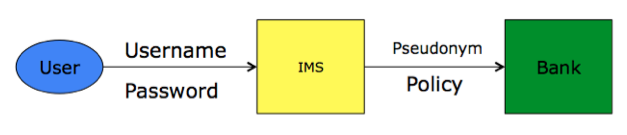
\includegraphics[width=\textwidth]{figures/Pseudonym}
	\caption{Prototype Design}
	\label{fig:Pseudonym}
\end{figure}
For end user it doesn't change anything. End user authenticates to the IMS and then IMS creates a pseudonym for the user. This pseudonym is then used by the bank for providing the services to the customer.
\section{Authentication}
\begin{figure}[h]
	\centering
	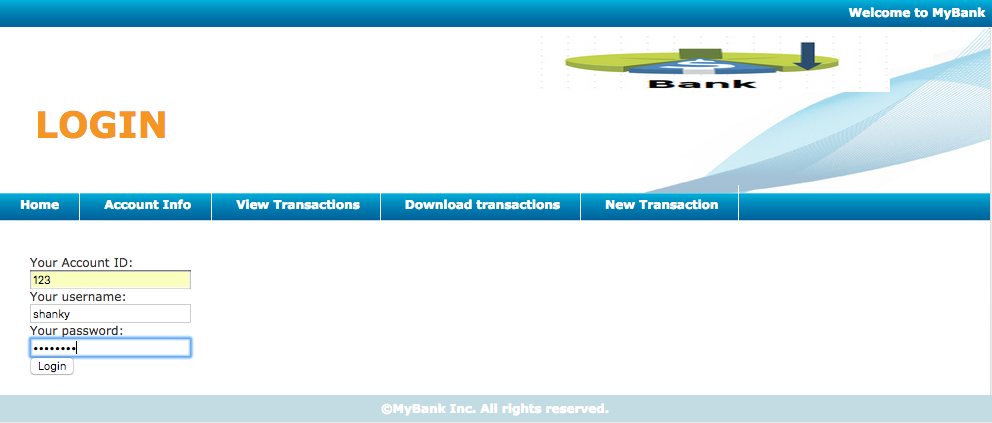
\includegraphics[width=\textwidth]{figures/Login}
	\caption{User Login Page}
	\label{fig:Login}
\end{figure}
\begin{figure}[h]
	\centering
	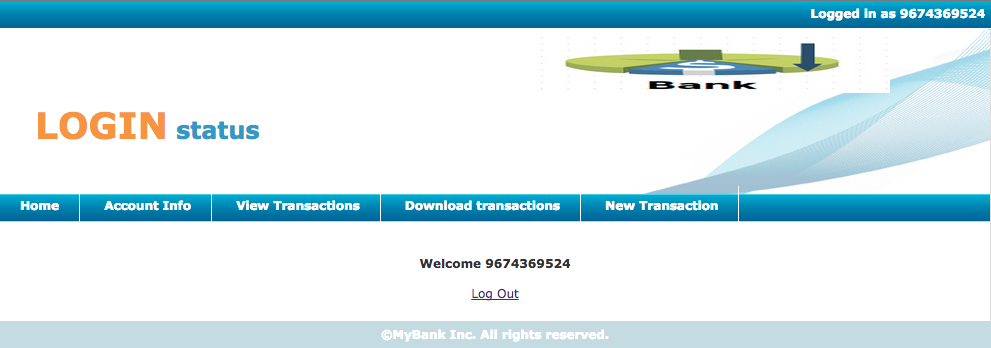
\includegraphics[width=\textwidth]{figures/Logged}
	\caption{Authenticated User}
	\label{fig:Logged}
\end{figure}	
User authentication happens as follows:
\begin{itemize}
	\item User goes to the bank login page.
	\item User puts his credentials in the login system.
	\item User credentials are verified by IMS and then user is redirected to his account page.
\end{itemize}
One thing to note that is that as traditional user, this doesn't change anything on the user end. User still use the same process to get access to his account.
\\
\\As we can see in \ref{fig:Logged}, after authentication user is logged in with a pseudonym.	
\section{User Information}
\begin{figure}[h]
	\centering
	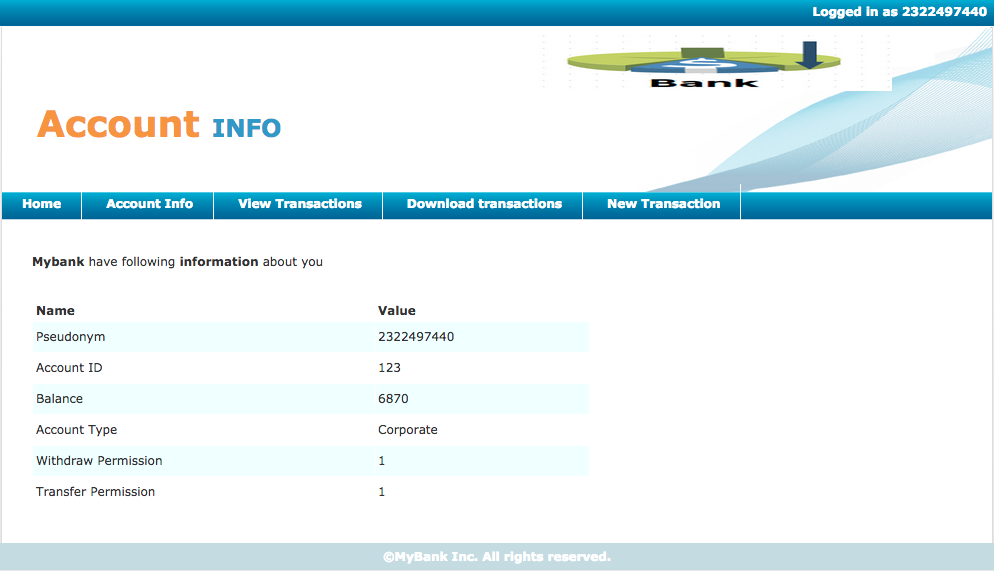
\includegraphics[width=\textwidth]{figures/Account1}
	\caption{User Information - Session 1}
	\label{fig:Account1}
\end{figure}	
\begin{figure}[h]
	\centering
	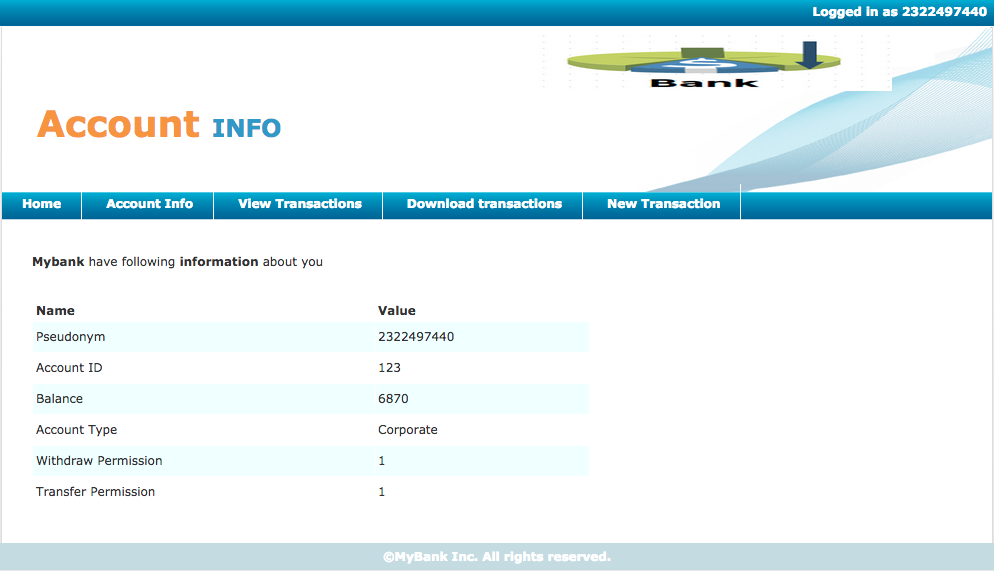
\includegraphics[width=\textwidth]{figures/Account1}
	\caption{User Information - Session 2}
	\label{fig:Account2}
\end{figure}
When we go to user information page we can see the information that is given to the bank by IMS for a given user.
\\
\\In our case it is:
\begin{itemize}
	\item Pseudonym
	\item Account ID
	\item Balance
	\item Account Type
	\item Policies
	\begin{itemize}
		\item Withdraw Permission
		\item Transfer Permission
	\end{itemize}
\end{itemize}
As we can see from \ref{fig:Account1} and \ref{fig:Account2}, 2 different sessions of the same user are logged in with different pseudonym. Bank have no way to find out that its the same user who have logged into different sessions.

\section{Transactions}
\begin{figure}
	\centering
	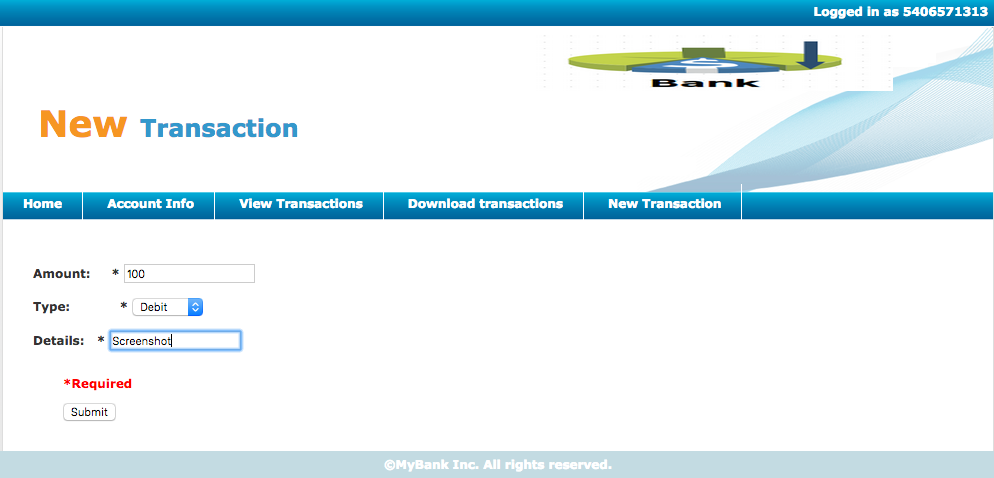
\includegraphics[width=\textwidth]{figures/New}
	\caption{New Transactions}
	\label{fig:New}
\end{figure}
In our prototype user is allowed to do 2 types of transactions
\begin{itemize}
	\item Debit
	\item Credit
\end{itemize}
All the transactions that are done by the user are logged in with the pseudonym; with which user has been logged in to the system.
\\
\\\ref{fig:New} shows the new transactions page in the system where user is allowed to do the transactions.
\begin{figure}[h]
		\centering
		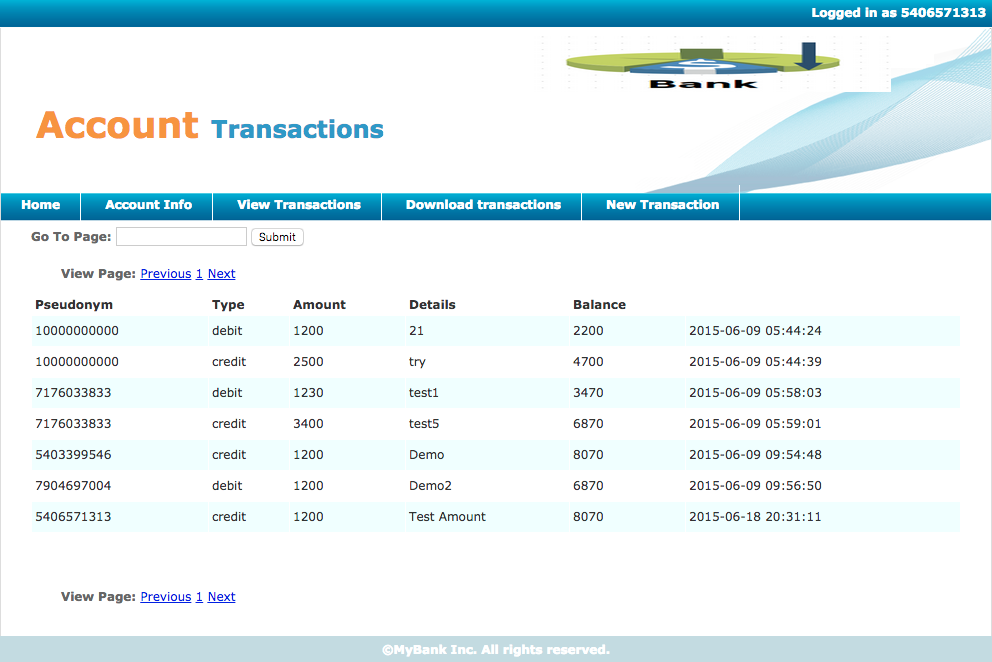
\includegraphics[width=\textwidth]{figures/Transactions}
		\caption{Account Transactions}
		\label{fig:Transactions}
\end{figure}
\\
\\\ref{fig:Transactions} shows all the transactions that has been done on the given account by users. As we can see, all the transactions are saved with the pseudonym of the users.
\begin{figure}[h]
	\centering
	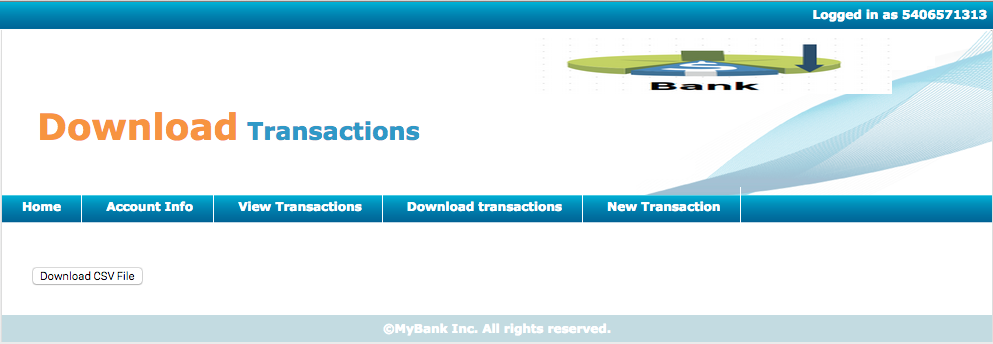
\includegraphics[width=\textwidth]{figures/Download}
	\caption{Download Transactions Option}
	\label{fig:Download}
\end{figure}
\begin{figure}[h]
	\centering
	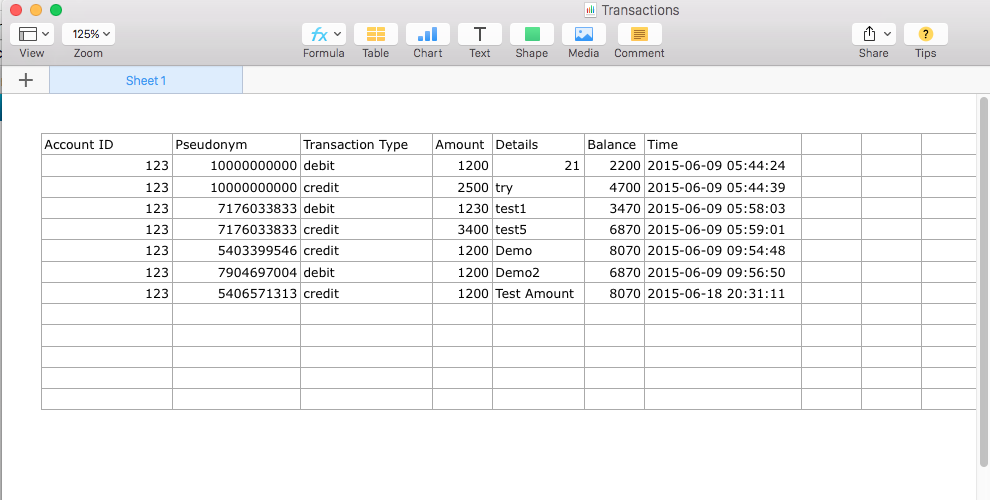
\includegraphics[width=\textwidth]{figures/File}
	\caption{Downloaded Transactions File}
	\label{fig:File}
\end{figure}	
\\
\\Our system also allow the users to download the transactions from the download transactions page as shown in \ref{fig:Download}. These transactions are stored in a csv file and then can be seen as in \ref{fig:File}.
\section{Summary}
In this chapter we showed a simple prototype of our system. This system works with pseudonyms and in the next chapter we will talk about how we can replace our Identity Mapping System with OpenID and IDEMIX for our purposes.